\documentclass[11pt,a4paper]{article}
\usepackage[margin=2.2cm]{geometry}
\usepackage{amsmath,amssymb}
\usepackage{graphicx}
\usepackage{booktabs}
\usepackage{float}
\usepackage{enumitem}
\usepackage[hidelinks]{hyperref}
\usepackage{xcolor}
\setlist{itemsep=2pt,topsep=4pt}
\newcommand{\R}{\mathbf{R}}
\newcommand{\tv}{\mathbf{t}}
\newcommand{\n}{\mathbf{n}}
\newcommand{\K}{\mathbf{K}}
\newcommand{\X}{\mathbf{X}}
\newcommand{\x}{\mathbf{x}}
\newenvironment{viva}{\par\medskip\noindent\colorbox{gray!12}{\parbox{\dimexpr\linewidth-2\fboxsep}{\textbf{If the professor asks.}\ }}\par\begingroup\itshape}{\endgroup\par\medskip}
\newcommand{\intuition}[1]{\par\noindent\textbf{Intuition.} #1\par\medskip}
\graphicspath{{../final/figures/}}

\title{Two-Image Pose Pipeline\\[2pt]\large Parts 9--12: decomposition, refinement, outputs and evaluation}
\author{Sai Svanik Chiramana (ME23B195) \and Sathwik Chanduluri (ME23B238)\\[2pt]\small CS6350 Computer Vision, TPA-12}
\date{}

\sloppy
\begin{document}
\maketitle

\noindent After Part 8 the pipeline has the inlier matches and one chosen model, a homography $H$ (flat object) or an essential matrix $E$ (any rigid object). Parts 9--12 turn that model into the final rotation and translation, polish it, report it with an error measure, and measure how good it is. Every number below is from our own runs with \emph{only the two images} (focal length estimated by MASt3R, object region found automatically), unless it says otherwise.

% =====================================================================
\section*{Part 9: Decomposition --- from $H$ or $E$ to one $(\R,\tv)$}

\textbf{In one line:} both $H$ and $E$ factor into several mathematically valid motions; we keep the one that is physically possible and best supported by all matches, and for flat objects we resolve a genuine two-way ambiguity.

\intuition{A model like $E$ only says ``the rays of every match meet somewhere''. Several motions produce exactly the same $E$: the camera could have moved forwards or backwards, and could have turned one way or the mirrored way. Only one of them puts the object \emph{in front of} both cameras. For a flat object there is a second, deeper ambiguity: two different tilts of the plane explain the images equally well.}

\subsection*{9.1 From $E$: four candidates and the cheirality test}
Write the singular value decomposition $E = U\,\mathrm{diag}(1,1,0)\,V^\top$ and
\[
W=\begin{pmatrix}0&-1&0\\1&0&0\\0&0&1\end{pmatrix}.
\]
Then the rotation is $\R = UWV^\top$ or $\R = UW^\top V^\top$, and the translation direction is $\tv=\pm\mathbf{u}_3$ (the last column of $U$). That gives four candidates $(\R,\pm\tv)$ for each $E$.

\textbf{Cheirality} (``handedness'') picks one: triangulate every inlier with each candidate and count how many 3D points have positive depth in \emph{both} cameras. A wrong candidate puts most points behind a camera. The winner is kept; OpenCV's \texttt{recoverPose} does this.

\emph{Triangulation} means finding the 3D point where the two viewing rays of a match (nearly) meet. With camera matrices $P_1=[I\,|\,0]$ and $P_2=[\R\,|\,\tv]$, each image point gives two linear equations in the unknown point; the four equations are solved by SVD (the linear method of Hartley \& Zisserman, \S12.2).

\subsection*{9.2 From $H$: up to four candidates, and the plane ambiguity}
In normalised coordinates the homography is $H_n = \K_2^{-1} H \K_1 = \R + \tv\,\n^\top/d$, where $\n$ is the plane normal and $d$ its distance. Decomposing $H_n$ (Malis \& Vargas) gives up to four solutions $(\R_i,\tv_i,\n_i)$. Removing those that put the matched points behind a camera leaves two, and for a perfectly flat scene \emph{both} reproduce the images exactly. We separate them, in order:
\begin{enumerate}
  \item \textbf{More points in front of both cameras} after triangulating the inliers.
  \item \textbf{Sampson error over all matches}, not just the plane's inliers. Real objects are never perfectly flat: points slightly off the plane fit only the true pose. Used only if one candidate is at least $1.5\times$ better.
  \item Otherwise a \textbf{prior}: the plane faces both cameras, i.e.\ score $|n_z| + |(\R\n)_z|$ (the normal points roughly along the viewing axis in both views), which is true when photographing an object's surface.
\end{enumerate}
\emph{Example:} one candidate has normal $\n=(0.1,0.0,0.99)$ (facing the camera), the other $\n=(0.7,0.0,0.71)$ (seen at $45^\circ$). If the Sampson errors are similar, the first wins.

\subsection*{9.3 The planar-twin check on $E$}
On a nearly flat object GRIC may still choose $E$ (the object is not perfectly flat), but $E$ is then weakly determined and can land on the \emph{wrong} one of the two plane solutions. On a book we saw $3^\circ$ reported for a true $28^\circ$. So whenever $E$ is chosen we also look at $H$'s decomposition:
\begin{enumerate}
  \item Find the $H$ candidate closest to the $E$ pose. If none is within $10^\circ$, the scene is not planar enough for the ambiguity to exist: keep $E$.
  \item Take its ``twin'': the other physically valid $H$ candidate (more than $2^\circ$ away).
  \item Replace the $E$ pose by the twin only if the twin explains \emph{all} matches nearly as well (median Sampson error at most $3\times$ the $E$ pose's), and either the Sampson error clearly prefers the twin ($1.5\times$) or, when it does not, the twin faces both cameras better.
  \item If the $E$ pose matches a candidate that the visibility test rules out, replace it by the best visible candidate (same fit condition).
\end{enumerate}
\textbf{Effect} (benchmark, same matches): it raised every matcher's mean AUC@10 by 1--3 points, XFeat+LightGlue on Objectron by 9 (49.3 $\to$ 58.2), and $E$ on distant flat posters from 5.8 to 18.6; no dataset lost more than 0.3. The thresholds ($10^\circ$, $3\times$) were chosen on the tuning split.

\begin{viva}
``$E$ and $H$ each factor into several motions. For $E$ we take the SVD, get four candidates, and keep the one that puts the triangulated points in front of both cameras. A plane has a genuine two-fold ambiguity, so for $H$ we break the tie with the Sampson error of all matches, since off-plane points fit only the true pose, and otherwise with the prior that the plane faces the camera. When $E$ is chosen on a nearly flat object, a planar-twin check swaps in the other plane solution if it fits better; that added 1--3 AUC points to every matcher.''
\end{viva}

\noindent\textbf{Sources.} Hartley \& Zisserman, \emph{Multiple View Geometry}, 2nd ed., 2004: \S9.6.2 (four solutions from $E$), \S12.2 (triangulation), ch.~13 (plane homographies). Malis \& Vargas, ``Deeper understanding of the homography decomposition for vision-based control'', INRIA RR-6303, 2007. Faugeras \& Lustman, ``Motion and structure from motion in a piecewise planar environment'', IJPRAI 2(3), 1988, and Longuet-Higgins, Proc.\ Royal Society B 227, 1986 (two solutions for a plane). OpenCV \texttt{recoverPose}, \texttt{decomposeHomographyMat}, \texttt{filterHomographyDecompByVisibleRefpoints}. \emph{Our own:} the three-step tie-break and the planar-twin check with its thresholds (\texttt{src/pipeline/geometry.py}).

% =====================================================================
\section*{Part 10: Refinement --- Levenberg--Marquardt}

\textbf{In one line:} the pose from MAGSAC++ is computed from tiny samples; refinement adjusts $\R$ and $\tv$ directly to minimise a pixel-level error over \emph{all} inliers, then re-selects the inliers and refines again.

\intuition{MAGSAC++ fits a model to 4 or 5 matches and polishes it with an algebraic error, which is convenient but not exactly ``how many pixels off''. With hundreds of inliers available, we can nudge the pose until every inlier fits as closely as possible in pixels, which averages out the noise of individual matches.}

\subsection*{10.1 Levenberg--Marquardt in brief}
Given residuals $\mathbf{r}(\theta)$ (one per inlier) and their Jacobian $J$, each step solves
\[
\big(J^\top J + \lambda\,\mathrm{diag}(J^\top J)\big)\,\delta = -J^\top \mathbf{r},\qquad \theta \leftarrow \theta + \delta .
\]
With small $\lambda$ this is Gauss--Newton (fast near the solution); with large $\lambda$ it becomes small gradient-descent steps (safe far from it). $\lambda$ is lowered after a successful step and raised after a failed one. We use SciPy's \texttt{least\_squares(method="lm")}, which wraps MINPACK.

\subsection*{10.2 What is optimised}
\begin{table}[H]\centering\small
\resizebox{\linewidth}{!}{\begin{tabular}{lll}
\toprule
 & $E$ model (any rigid object) & $H$ model (flat object)\\
\midrule
Parameters & $\R$: 3 (rotation vector, $\R=\mathrm{Rod}(\mathbf{w})\R_0$) & $\R$: 3, $\tv/d$: 3, $\n$: 2 (on the unit sphere)\\
 & $\tv$ direction: 2 (moves on the unit sphere) & = 8, as many as a homography\\
Residual per inlier & signed Sampson distance (px) & symmetric transfer error of $\K_2(\R+\tv\n^\top/d)\K_1^{-1}$\\
\bottomrule
\end{tabular}}
\end{table}
\noindent The translation stays a unit vector by moving it in the plane tangent to the sphere and renormalising: $\tv = (\tv_0 + B\mathbf{x})/\|\tv_0 + B\mathbf{x}\|$, with $B$ two vectors orthogonal to $\tv_0$. The Sampson distance is the first-order approximation of the true reprojection error, so no 3D point has to be estimated. For $H$, the refined result is still a rigid motion seen through a plane, never an arbitrary $3\times3$ matrix.

\subsection*{10.3 Safeguards and inlier re-selection}
\begin{enumerate}
  \item Keep the refined pose only if the \emph{median} residual went down (LM can drift when inliers are few or nearly degenerate); at least 8 inliers are needed.
  \item With the refined pose, re-test \emph{all} matches against the 1.5\,px threshold: some that MAGSAC++ rejected now fit.
  \item Refine again on the new inlier set (at most 2 rounds); stop if the set shrinks or does not change.
\end{enumerate}

\begin{viva}
``After robust fitting we refine the pose with Levenberg--Marquardt over all inliers: for $E$ we optimise the rotation and the translation direction on the unit sphere to minimise the Sampson distance, and for $H$ the rotation, translation over depth and plane normal to minimise the transfer error. Then we re-select inliers with the refined pose and refine once more, keeping the result only if the median error drops.''
\end{viva}

\noindent\textbf{Sources.} Levenberg, Quarterly of Applied Mathematics 2, 1944; Marquardt, SIAM J.\ Applied Mathematics 11, 1963; Mor\'e, ``The Levenberg--Marquardt algorithm: implementation and theory'', Numerical Analysis, Springer LNM 630, 1978 (MINPACK). Hartley \& Zisserman, Appendix~6 (iterative estimation) and \S11.4.3 (Sampson distance). Virtanen et al., ``SciPy 1.0'', Nature Methods 17, 2020. \emph{Our own:} the parameterisations, the median safeguard and the two-round re-selection (\texttt{src/pipeline/refine.py}).

% =====================================================================
\section*{Part 11: Reprojection error, fallback retry and verdict}

\textbf{In one line:} we report the RMS reprojection error that the task asks for, retry on the whole image if the object region gave too little, and add a verdict that flags results the numbers alone cannot vouch for.

\subsection*{11.1 How the reprojection error is computed}
\begin{enumerate}
  \item Triangulate each inlier $(\mathbf{p}_1,\mathbf{p}_2)$ with the final $\K_1,\K_2,\R,\tv$ (Part 9) to a 3D point $\X$.
  \item Keep points with positive depth in both cameras.
  \item Project $\X$ back: $\hat{\mathbf{p}}_1 = \pi(\K_1\X)$, $\hat{\mathbf{p}}_2=\pi(\K_2(\R\X+\tv))$, where $\pi$ divides by the third coordinate.
  \item Report
  \[
  \text{RMS} = \sqrt{\tfrac{1}{2N}\textstyle\sum_{i=1}^{N}\big(\|\hat{\mathbf{p}}_{1,i}-\mathbf{p}_{1,i}\|^2 + \|\hat{\mathbf{p}}_{2,i}-\mathbf{p}_{2,i}\|^2\big)}\quad\text{(pixels)}.
  \]
\end{enumerate}
On our 56 test pairs the median is 0.46\,px for MASt3R (0.32\,px with the true $\K$ and mask).

\subsection*{11.2 Why a low reprojection error does not prove the pose is right}
The error measures \emph{consistency}: whether one rigid motion explains the inliers. A wrong but self-consistent answer scores just as well, for example the other solution of a planar object, or a pose computed on the wrong region. Figure~\ref{fig:fail} is our worst case: the region finder paired the cardboard strip on the right of the board in image 1 with the strip on the left in image 2. MASt3R matched them consistently, and the pose is $61.7^\circ$ wrong with an RMS of only 0.49\,px.

\begin{figure}[H]\centering
\includegraphics[width=\linewidth]{case_failure.png}
\caption{Failure case (TUM checkerboard, true rotation $16.8^\circ$): wrong counterpart regions give a confident but wrong pose. Rotation error $61.7^\circ$, reprojection RMS 0.49\,px.}
\label{fig:fail}
\end{figure}

\subsection*{11.3 Fallback retry}
If the pose fails on an automatically found region (fewer than 15 matches or inliers) and that region was ``moved'' or ``unconfirmed'', the pose is recomputed on the whole images. The verdict then says the result is the camera's motion relative to the scene.

\subsection*{11.4 The verdict}
\begin{table}[H]\centering\small
\resizebox{\linewidth}{!}{\begin{tabular}{ll}
\toprule
Verdict & When\\
\midrule
\textsc{no result} & nothing could be fitted, or only the outline stage answered on a box-shaped mask\\
\textsc{uncertain} & fewer than 30 inliers; reprojection RMS above 2\,px; rotation above $60^\circ$ with a 2D matcher;\\
 & or the focal length is only the $70^\circ$ guess\\
\textsc{scene motion only} & whole images used (``scene'' or ``none'' region): camera motion relative to the scene\\
\textsc{reliable} & none of the above; notes say whether the object was confirmed by motion\\
\bottomrule
\end{tabular}}
\end{table}

\subsection*{11.5 How well do these indicators work?}
\begin{itemize}
  \item \textbf{Verdict} (MASt3R, 56 test pairs): \textsc{reliable} on 16 pairs, median pose error $3.0^\circ$, 2 of 16 above $20^\circ$; \textsc{scene} on 39 pairs, median $2.2^\circ$. It catches some failures but not wrong-but-consistent ones.
  \item \textbf{Two-method agreement} (new): the angle between the MASt3R rotation and the \texttt{accurate} rotation. When they agree within $2^\circ$ (34 pairs), \emph{none} of MASt3R's rotations was more than $10^\circ$ off; when they disagree, 14\% were. Two independent matchers are unlikely to be wrong in the same way, so agreement is a strong indicator of a correct rotation. It does not predict translation errors, which on near-identical frames are large for every method.
\end{itemize}

\subsection*{11.6 Metric translation (optional)}
Two images give $\tv$ only as a direction. With \texttt{--size} (the object's longest dimension), the triangulated inliers' extent along their main axis is matched to that length; on Objectron this recovers $|\tv|$ with a median error of 17.9\% (benchmark with dataset $\K$).

\begin{viva}
``We triangulate the inliers with the final pose, project them back into both images and report the RMS pixel error, as the task asks. It shows the answer is self-consistent, not that it is correct, so we also give a verdict, and we found that agreement between two independent matchers is a much better sign: when MASt3R and our SIFT/XFeat cascade agree within two degrees, MASt3R's rotation was never more than ten degrees off.''
\end{viva}

\noindent\textbf{Sources.} Hartley \& Zisserman, \S12.2 (triangulation) and ch.~4 (reprojection error). \emph{Our own:} the fallback retry, the verdict rules, the agreement check and the size-based scale (\texttt{auto\_run.py}, \texttt{src/pipeline/geometry.py}, \texttt{src/pipeline/scale.py}).

% =====================================================================
\section*{Part 12: Evaluation and results}

\textbf{In one line:} on 56 held-out pairs with only the two images, MASt3R reaches a median rotation error of $0.97^\circ$ and translation-direction error of $1.79^\circ$, within one AUC point of the same method given the true camera and mask.

\subsection*{12.1 Metrics}
\begin{itemize}
  \item \textbf{Rotation error} (geodesic): $e_R = \arccos\big((\mathrm{tr}(\R_{est}^\top\R_{gt})-1)/2\big)$, the angle of the rotation still needed to reach the truth. Unlike per-axis Euler errors it does not depend on an axis order.
  \item \textbf{Translation-direction error}: $e_t = \arccos\big(\tv_{est}^\top\tv_{gt}/(\|\tv_{est}\|\|\tv_{gt}\|)\big)$; scale is not observable.
  \item \textbf{Pose error} $=\max(e_R, e_t)$: a pose counts as good only if both parts are good.
  \item \textbf{AUC@$\tau$}: plot the fraction of pairs whose pose error is below $x$, for $x$ from 0 to $\tau$ ($5^\circ$, $10^\circ$, $20^\circ$); the area under that curve, as a percentage of $\tau$. A method that is always perfect scores 100. \emph{Failures count as infinite error}, so refusing hard pairs is never rewarded. This is the standard measure of SuperGlue and LoFTR.
  \item For comparison with CS6350.pdf: per-axis roll/pitch/yaw errors and their MAE, MSE, MAX, MIN, STD.
\end{itemize}

\subsection*{12.2 Test design}
\begin{itemize}
  \item \textbf{Data:} TUM RGB-D (5 sequences: posters, 3D structures, checkerboard), Objectron (book, laptop, cereal box), CO3D (phone, handbag), MVImgNet (key, watch); 12 objects and scenes, 7 near-planar and 5 three-dimensional.
  \item \textbf{Split:} every threshold, including the region rule, was chosen on tuning sequences only; results are from held-out test sequences.
  \item \textbf{Pairs:} 32 main pairs (one per object and viewpoint bin: 5--15, 15--30, 30--60$^\circ$), 10 consecutive-frame TUM pairs (under $1^\circ$), 14 pairs at 60--90$^\circ$.
  \item \textbf{Methods:} MASt3R (default), \texttt{confident}, \texttt{accurate}; reference: MASt3R with the dataset's $\K$ and region.
\end{itemize}

\subsection*{12.3 Results}
\begin{table}[H]\centering\small
\begin{tabular}{lcccccc}
\toprule
Method (two images only) & AUC@5/10/20 & med.\ $e_R$ & med.\ $e_t$ & med.\ reproj. & $>20^\circ$ off & s/pair\\
\midrule
MASt3R & 41.4 / \textbf{57.5} / 68.9 & \textbf{0.97}$^\circ$ & 1.79$^\circ$ & \textbf{0.46}\,px & 18\% & 15.5\\
\texttt{confident} & 40.5 / 55.2 / 65.7 & 1.07$^\circ$ & \textbf{1.74}$^\circ$ & 0.63\,px & 23\% & 0.6\\
\texttt{accurate} & 30.7 / 39.8 / 47.3 & 1.57$^\circ$ & 7.79$^\circ$ & 0.77\,px & 45\% & 0.6\\
\midrule
\emph{reference: true $\K$ + mask} & 44.4 / 58.5 / 69.7 & 0.72$^\circ$ & 2.20$^\circ$ & 0.32\,px & 18\% & --\\
\bottomrule
\end{tabular}
\caption{All 56 test pairs. Median seconds exclude the focal and region steps (about 40\,s and 25\,s, shared by all methods).}
\end{table}

\begin{table}[H]\centering\small
\resizebox{\linewidth}{!}{\begin{tabular}{lcccccc}
\toprule
Viewpoint change & pairs & MASt3R AUC@10 & \texttt{confident} & \texttt{accurate} & MASt3R med.\ $e_R$ & MASt3R med.\ $e_t$\\
\midrule
under $1^\circ$ (consecutive) & 10 & 7.4 & 7.4 & 0.0 & 0.32$^\circ$ & 44.6$^\circ$\\
5--15$^\circ$ & 12 & 70.9 & 72.3 & 68.2 & 0.76$^\circ$ & 1.65$^\circ$\\
15--30$^\circ$ & 11 & 80.3 & 71.3 & 71.3 & 1.11$^\circ$ & 0.78$^\circ$\\
30--60$^\circ$ & 9 & 68.8 & 59.5 & 53.0 & 1.68$^\circ$ & 1.77$^\circ$\\
60--90$^\circ$ & 14 & 65.2 & 67.8 & 17.2 & 3.08$^\circ$ & 1.41$^\circ$\\
\bottomrule
\end{tabular}}
\caption{By viewpoint change. On consecutive frames the rotation is excellent but the translation direction is not observable (the camera moves millimetres), so the AUC, which needs both, is low for every method.}
\end{table}

\begin{table}[H]\centering\small
\begin{tabular}{lcc}
\toprule
 & planar (32 pairs) & 3D (24 pairs)\\
\midrule
MASt3R AUC@10 & 56.1 & 61.1\\
\texttt{accurate} AUC@10 & 32.5 & 51.5\\
\bottomrule
\end{tabular}\qquad
\begin{tabular}{lcc}
\toprule
MASt3R & before fix & after fix\\
\midrule
AUC@10 & 50.2 & \textbf{57.5}\\
med.\ $e_R$ & 1.27$^\circ$ & \textbf{0.97}$^\circ$\\
pairs $>20^\circ$ off & 25\% & \textbf{18\%}\\
\bottomrule
\end{tabular}
\caption{Left: planar vs 3D objects. Right: effect of the region-rule fix (version 2, tuned on the tuning split), same 56 test pairs.}
\end{table}

\begin{figure}[H]\centering
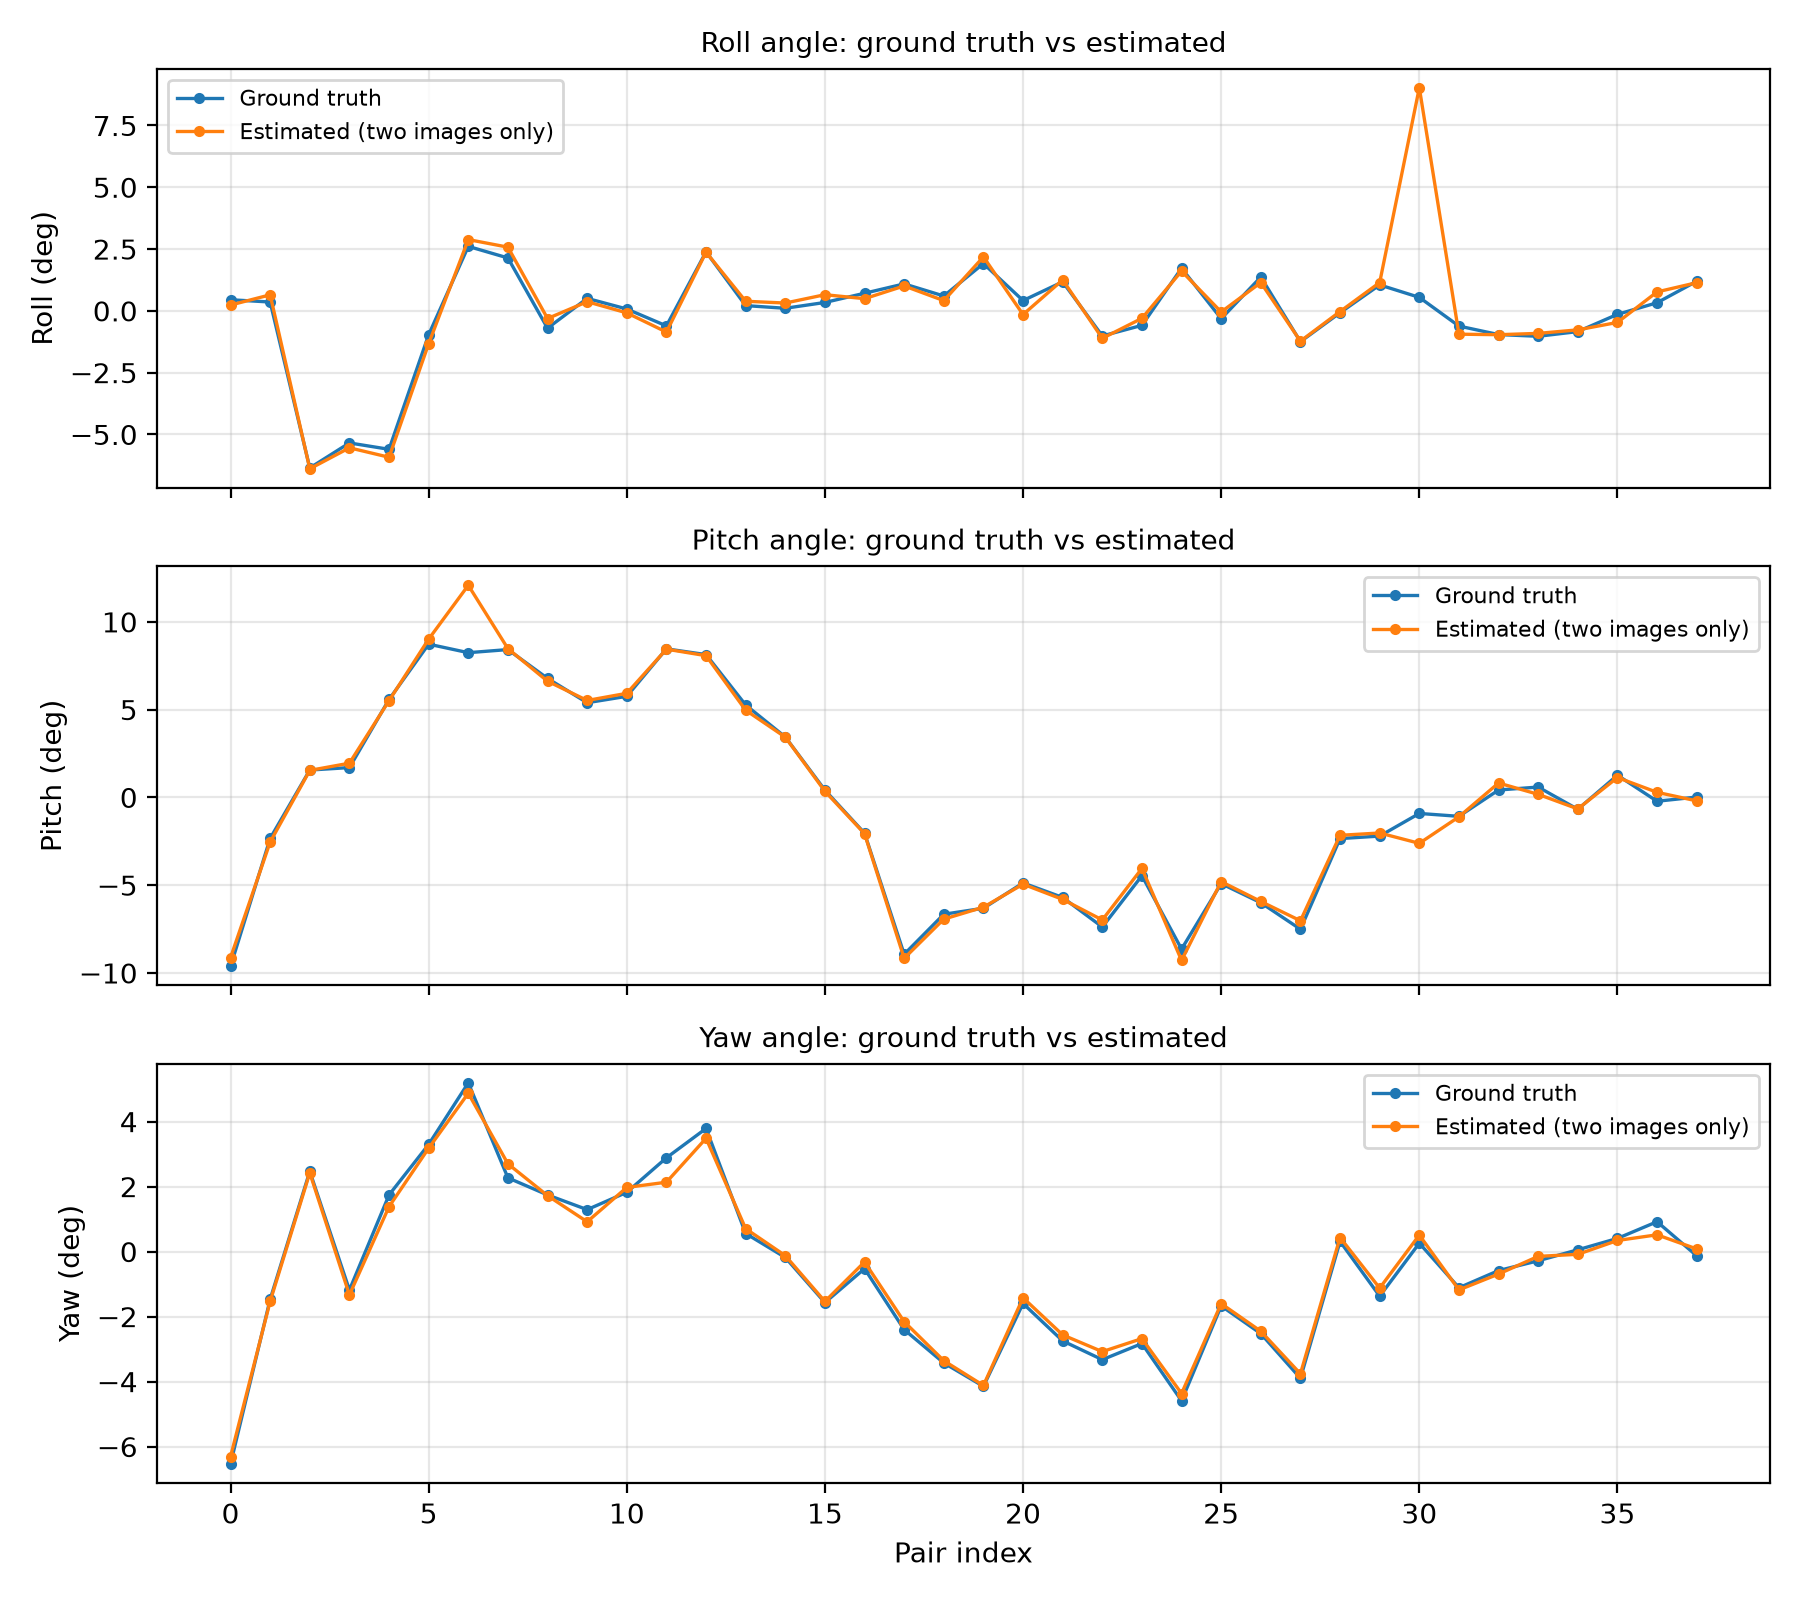
\includegraphics[width=0.82\linewidth]{euler_struct_near_gap20.png}
\caption{Frame-wise roll, pitch and yaw against ground truth: 38 TUM \texttt{struct\_near} pairs 20 frames apart, each solved from the two images only (the counterpart of CS6350.pdf, Fig.~13). Per-axis MAE $0.43^\circ$ / $0.34^\circ$ / $0.19^\circ$.}
\label{fig:euler}
\end{figure}

\begin{table}[H]\centering\small
\resizebox{\linewidth}{!}{\begin{tabular}{lcccc}
\toprule
 & \multicolumn{2}{c}{small motion (consecutive frames)} & \multicolumn{2}{c}{larger motion (20 frames / 5--15$^\circ$)}\\
\cmidrule(lr){2-3}\cmidrule(lr){4-5}
Mean absolute error & CS6350 & \textbf{ours} & CS6350 & \textbf{ours}\\
\midrule
Rotation, average of roll/pitch/yaw & 0.229$^\circ$ & \textbf{0.195}$^\circ$ & 1.106$^\circ$ & \textbf{0.32}$^\circ$\,/\,\textbf{0.47}$^\circ$\\
Translation direction & 57.5$^\circ$ & \textbf{48.0}$^\circ$ & 64.7$^\circ$ & \textbf{8.4}$^\circ$\,/\,\textbf{3.7}$^\circ$\\
Reprojection RMS & 1.03\,px & \textbf{0.22}\,px & 0.59\,px & \textbf{0.21}\,px\,/\,\textbf{0.37}\,px\\
Pairs & 100 & 10 & 100 & 38\,/\,12\\
\bottomrule
\end{tabular}}
\caption{Against CS6350.pdf (one TUM cabinet sequence, homography only, $f=\max(W,H)$). ``Ours'' larger motion: Euler track (Fig.~\ref{fig:euler}) / the 12 main pairs at 5--15$^\circ$. Different sequences, so indicative, not like for like.}
\end{table}

\subsection*{12.4 What the results say}
\begin{itemize}
  \item With only two images the pipeline is within one AUC point of the same method given the true camera and object mask: estimating the focal length and finding the object cost almost nothing on average.
  \item MASt3R is the best matcher overall and holds up to 60--90$^\circ$ (median $3.1^\circ$), where the 2D cascade fails on most pairs; \texttt{confident} matches it there by handing those pairs to MASt3R.
  \item Translation direction is recovered to about $2^\circ$ wherever the camera actually moves; CS6350's homography-only pipeline could not recover it ($57$--$65^\circ$).
  \item Remaining failures: wrong region pairing in static scenes (Figure~\ref{fig:fail}), unobservable translation on near-identical frames, and the focal estimate on close-ups.
\end{itemize}

\begin{viva}
``We measure the geodesic rotation error and the angle between translation directions, take the larger as the pose error, and report AUC at 5, 10 and 20 degrees with failures counted as infinite error. On 56 held-out pairs from four datasets, with only the two images, MASt3R gets a median rotation error under one degree and translation error under two degrees, within one AUC point of having the true camera and mask. Compared with CS6350's pipeline, rotation is as good or better and the translation-direction error is roughly 8 to 17 times smaller.''
\end{viva}

\noindent\textbf{Sources.} Hartley et al., ``Rotation Averaging'', IJCV 103, 2013 (geodesic distance). Sarlin et al., ``SuperGlue'', CVPR 2020, and Sun et al., ``LoFTR'', CVPR 2021 (pose AUC). Sturm et al., ``A benchmark for the evaluation of RGB-D SLAM systems'', IROS 2012; Ahmadyan et al., ``Objectron'', CVPR 2021; Reizenstein et al., ``Common Objects in 3D'', ICCV 2021; Yu et al., ``MVImgNet'', CVPR 2023. CS6350.pdf, Tables 1--2 and Fig.~13. \emph{Our own:} the test design, the bins and every number in this part (\texttt{scripts/auto\_eval.py}, \texttt{auto\_eval2.py}, \texttt{euler\_track.py}).

\end{document}
